\documentclass[12pt]{article}
\usepackage{csquotes}
\usepackage{amsmath,amsfonts,amssymb}
\usepackage{geometry}
\usepackage{pifont}
\usepackage[utf8]{inputenc}
\usepackage[english]{babel}
\usepackage{ragged2e}
\usepackage{blindtext}
\usepackage[backend=biber, style=numeric]{biblatex}
\usepackage[hyperindex,breaklinks,colorlinks=true,linkcolor=blue,citecolor=blue,urlcolor=blue]{hyperref}
\usepackage{tikz}

\addbibresource{references.bib}
\addbibresource{references/DolevReference.bib}
\addbibresource{references/ShirelReference.bib}
\addbibresource{references/HadasReference.bib}
\addbibresource{references/RoyReference.bib}
\addbibresource{references/MoriaReference.bib}

\geometry{a4paper, margin=1in}

\title{\textbf{Analysis of High-Dimensional Data}}
\author{
    Dolev Dublon - 207867342 |
    Moria Grohar - 323082024 \\
    Shirel Zecharia - 211551072 | 
    Roy Harel - 213055601 \\
    Hadas Evers - 206398984  
}
\date{\today}

\begin{document}

\maketitle


\tableofcontents

\newpage

\begin{abstract}
    This Survey explores the fascinating world of high-dimensional data analysis, focusing on the properties of random matrices. These matrices play a crucial role in various fields such as computer science, statistics, and machine learning, especially concerning their singularity and the analysis of their smallest singular values.
\end{abstract}

\section{Introduction}


In the realm of high-dimensional data analysis, random matrices have captivated the attention of mathematicians and scientists due to their ubiquitous presence in various domains, including computer science, statistics, and machine learning. Understanding their behavior is paramount, particularly regarding their singularity (non-invertibility) and the analysis of their smallest singular values. This article delves into ten research papers that shed light on these aspects.


\section{Chronological Order}

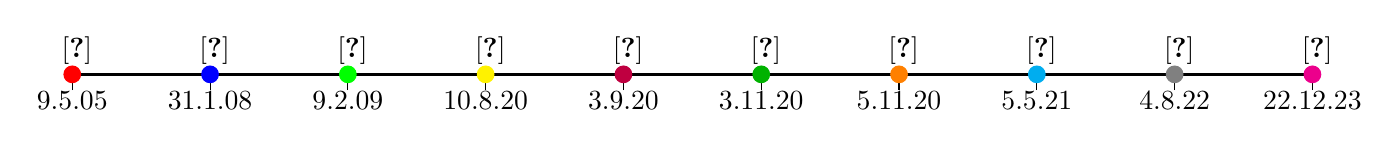
\begin{tikzpicture}
    \draw[line width=1pt] (0,0) -- (15.75,0);
    \foreach \x/\year in {0/9.5.05, 1.75/31.1.08, 3.5/9.2.09, 5.25/10.8.20, 7/3.9.20, 8.75/3.11.20, 10.5/5.11.20, 12.25/5.5.21, 14/4.8.22, 15.75/22.12.23} {
            \draw (\x,-0.2) -- (\x,0.1);
            \node[below] at (\x,-0.1) {\year};
        }
    % Articles
    \draw[red, fill=red] (0,0) circle (3pt) node[above, black] {~\cite{costello2005random}};
    \draw[blue, fill=blue] (1.75,0) circle (3pt) node[above, black] {~\cite{rudelson2008littlewood}};
    \draw[green, fill=green] (3.5,0) circle (3pt) node[above, black] {~\cite{costello2009bilinear}};
    \draw[yellow, fill=yellow] (5.25,0) circle (3pt) node[above, black] {~\cite{kwan2019algebraic}};
    \draw[purple, fill=purple] (7,0) circle (3pt) node[above, black] {~\cite{jain2020smoothed}};
    \draw[black!30!green, fill=black!30!green] (8.75,0) circle (3pt) node[above, black] {~\cite{jain2020smallest}};
    \draw[orange, fill=orange] (10.5,0) circle (3pt) node[above, black] {~\cite{campos2020singularity}};
    \draw[cyan, fill=cyan] (12.25,0) circle (3pt) node[above, black] {~\cite{jain2021singularity}};
    \draw[black!50, fill=black!50] (14,0) circle (3pt) node[above, black] {~\cite{kwan2022anticoncentration}};
    \draw[magenta, fill=magenta] (15.75,0) circle (3pt) node[above, black] {~\cite{kwan2023resolution}};
\end{tikzpicture}


\section{Random Matrices and Singularity}
The study of the singularity of random matrices is crucial because it directly impacts our understanding of system behaviors, algorithmic stability, and numerical methods across various disciplines. 
Singular matrices, which lack inverses, highlight dependencies and potential points of failure in systems and calculations (these dependencies could indicate redundancy in data, or reveal vulnerabilities in cryptographic systems). 
Investigating these singularities in random matrices helps ensure the reliability and efficiency of computational approaches, contributing significantly to advancements in theoretical and applied mathematics.


\subsection{Random Symmetric Matrices Are Almost Surely Non-Singular}



"Random Symmetric Matrices Are Almost Surely Non-Singular" by Costello, Tao, and Vu (\cite{costello2005random}) proves that symmetric random matrices \(Q_n\) with i.i.d. Bernoulli entries above the diagonal are almost surely non-singular. The non-singularity holds with probability \(1-O(n^{-1/8+\delta})\) for any \(\delta>0\), broadening earlier findings to a wider class of random matrices.
The article delves into the history of non-singularity in random matrices, focusing on whether matrices like \(A_n\) with independent Bernoulli variables are almost surely non-singular. Komlós affirmed this in 1967 and later extended his findings. Tao and Vu, in a more recent work, introduced a novel proof offering a precise determinant estimate for \(A_n\), enriching the understanding of random matrix non-singularity.
Building upon prior work, the authors propose a quadratic Littlewood-Offord theory to ascertain \(Q_n\)'s non-singularity, a symmetric matrix with i.i.d. Bernoulli variables. This approach addresses challenges like row and column transposition dependency. Attempting to linearize the quadratic \( Q=\sum_{1\leq i,j\leq n} c_{ij} z_i z_j \) into \( Q=\sum_{i=1}^n Q_i z_i \) revealed dependencies among \( Q_i \) coefficients on \( z_i \). To navigate this, "decoupling" was employed, refining the theoretical framework for random matrices' invertibility analysis.
\textbf{Decoupling lemma:} Given random variables \(X\) and \(Y\), and an event \(E=E(X,Y)\) dependent on \(X\) and \(Y\), then:
\[
P(E(X,Y)) \leq (P(E(X,Y) \land E(X',Y) \land E(X,Y') \land E(X',Y')))^{1/4}
\]
where \(X'\) and \(Y'\) are independent copies of \(X\) and \(Y\), respectively. This technique finds application across various domains, including graph theory.
The article outlines open questions for future research in random matrices:
\begin{itemize}
    \item \textbf{Determinant Estimation:} It questions how to estimate the determinant of random matrices, providing an initial estimate: \( |\det(Q_n)| = n^{1/2-o(1)} \).
    \item \textbf{Singularity Probability:} It seeks to refine the estimation of the probability that a random matrix is singular, estimating \( Q_n \)'s singularity probability as \( (1/2+o(1))^n \).
\end{itemize}
\vspace{\baselineskip}
\textbf{The quadratic variant of the Littlewood-Offord:}
Let \( Q \) be a quadratic random variable defined as:
\vspace{-0.8\baselineskip}
\[ Q = \sum_{1 \leq i,j \leq n} c_{ij} z_i z_j \vspace{-0.5\baselineskip} \]
where \( z_i \) are random variables, \( \{1,\ldots,n\} = U_1 \cup U_2 \) is a non-trivial partition, and \( S \) is a non-empty subset of \( U_1 \). For each \( i \in S \), let \( d_i \) be the number of indices \( j \in U_2 \) such that \( |c_{ij}| \geq 1 \). If \( d_i \geq 1 \) for each \( i \in S \), and \( I \) is an interval of length 1, then:
\vspace{-0.9\baselineskip}
\[ P(Q \in I) = O\left( |S|^{-1/2} + |S|^{-1} \sum_{i \in S} d_i^{-1/2} \right)^{1/4} \]




\subsection{The Littlewood-Offord problem and invertibility of random matrices}
Mark Rudelson and Roman Vershynin's work~\cite{rudelson2008littlewood} develops a general approach to the invertibility of random matrices, aiming to proves two basic conjectures on the distribution of the smallest singular value of random \(n \times n\) matrices with independent entries.\\\newline
\textbf{Theorem 1.1 (Invertibility: fourth moment).} Let \(A\) be an \(n \times n\) matrix whose entries are independent real random variables with variances at least \(1\) and fourth moments bounded by \(B\). Then, for every \(\delta > 0\) there exist \(\epsilon > 0\) and \(n_0\) which depend (polynomially) only on \(\delta\) and \(B\), and such that
\begin{equation*}
    [P(s_n(A) \leq \epsilon n^{-1/2}) \leq \delta] \text{ for all } (n \geq n_0).\\
\end{equation*}
\textbf{Theorem 1.2 (Invertibility: subgaussian).} Let \(\xi_1, \ldots, \xi_n\) be independent centered real random variables with variances at least \(1\) and subgaussian moments bounded by \(B\). Let \(A\) be an \(n \times n\) matrix whose rows are independent copies of the random vector \((\xi_1, \ldots, \xi_n)\). Then for every \(\epsilon \geq 0\) one has
\begin{equation*}
    [P(s_n(A) \leq \epsilon n^{-1/2}) \leq C\epsilon + c^n,] \text{ where } (C > 0) \text{ and } (c \in (0, 1)) 
\end{equation*}
depend (polynomially) only on B.
They prove both theorems using the inverse Littlewood-Offord problem. Inspired by Tau and Vu's recently proposed method to reduce the small ball probability to an arbitrary polynomial order by looking at the inverse problem:\\\newline
\textbf{Theorem 1.3 (Tao, Vu).} Let \(a_1, \ldots, a_n\) be integers, and let \(A \geq 1\), \(\epsilon \in (0, 1)\). Suppose for the random sign-sums one has
\[p_0(a) \geq n^{-A}.\]
Then all except \(O_{A,\epsilon}(n^{\epsilon})\) coefficients \(a_k\) are contained in the Minkowski sum of \(O\left(\frac{A}{\epsilon}\right)\) arithmetic progressions of lengths \(n^{O_{A,\epsilon}(1)}\).\\
Rudelson and Vershynin demonstrate that a similar phenomenon holds for real rather than integer numbers ak, for the small ball probabilities \(p_{\epsilon}(a)\) rather than the probability \(p_{0}(a)\) of exact values, and for general random sums rather than the random sign-sums.\\\newline
\textbf{Theorem 1.5 (Small Ball Probability).} Let \(\xi_1, \ldots, \xi_n\) be independent identically distributed centered random variables with variances at least \(1\) and third moments bounded by \(B\). Let \(a = (a_1, \ldots, a_n)\) be a vector of real coefficients such that, for some \(K_1, K_2 > 0\) one has
\[K_1 \leq |a_k| \leq K_2 \quad \text{for all } k.\]
Let \(\alpha \in (0, 1)\) and \(\kappa \in (0, n)\). Then for every \(\epsilon \geq 0\) one has
\[p_{\epsilon}(a) \leq \frac{C\sqrt{\kappa}}{\left(\epsilon + \frac{1}{D_{\alpha,\kappa}(a)}\right)} + C e^{-c\alpha^2\kappa},\]
where \(C, c > 0\) depend (polynomially) only on \(B, K_1, K_2\).\\
Theorem 1.5 can also be restated as an inverse Littlewood-Offord theorem:\\\newline
\textbf{Corollary 1.6 (Inverse Littlewood-Offord Theorem).} Let \(a_1, \ldots, a_n\) be real numbers satisfying (1.11) and \(\xi_1, \ldots, \xi_n\) be random variables as in Theorem 1.5. Let \(A \geq \frac{1}{2}\), \(\kappa \in (0, n)\) and \(\epsilon > 0\). Suppose for the random sums (1.8) one has
\[p_\epsilon(a) \geq n^{-A}.\]
Then there exists an arithmetic progression of length \(L = O(n^{A\kappa^{-1/2}})\) and with gap between its elements \(d \leq 1\), and such that all except \(\kappa\) coefficients \(a_k\) are within distance \(O\left(\frac{A \log(n)}{\kappa}\right)^{1/2} \cdot d\) from the elements of the progression, provided that \(\epsilon \leq \frac{1}{L}\).\\
Their proof for Theorem 1.5 utilizes Halász's method to assess the probability of small deviations by examining a vector's recurrence to an integer lattice. The technique leverages density arguments to show that closeness to distinct lattice points in a short timeframe implies a small least common denominator (LCD) for the vector, indicating a strong structural property of the vector in question.\\
The paper's main result, the Strong Invertibility Theorem 5.1, reduces estimating the smallest singular value of random matrices
to estimating the largest singular value, which is used to imply both Theorems 1.1 and 1.2.\\\newline
\textbf{Theorem 5.1 (Strong invertibility).} Let \(\xi_1, \ldots, \xi_n\) be independent centered random variables with variances at least \(1\) and fourth moments at most \(B\). Let \(A\) be an \(n \times n\) matrix whose rows are independent copies of the random vector \((\xi_1, \ldots, \xi_n)\). Let \(K \geq 1\). Then for every \(\epsilon \geq 0\) one has
\[P(s_n(A) \leq \epsilon n^{-1/2}) \leq C\epsilon + c^n + P(\|A\| > K n^{1/2}),\]
where \(C > 0\) and \(c \in (0, 1)\) depend (polynomially) only on \(B\) and \(K\).\\
The general approach to invertibility of random matrices is developed in two stages. Initially, a "soft" argument, utilizing the central limit theorem, yields a basic result, which applies to both the Fourth Moment Theorem 1.1 and a weaker version of the Subgaussian Theorem 1.2. Later developing it into the Strong Invertibility Theorem 5.1 using the Small Ball Probability Theorem 1.5 instead of the central limit theorem.\\
The paper details a two-pronged strategy for demonstrating the invertibility of matrices by examining their behavior with different types of vectors: compressible and incompressible.
For compressible vectors, whose significant components are few, the analysis simplifies by focusing on a submatrix of the original, leveraging known results about the smallest singular value of random matrices.
In contrast, the invertibility for incompressible vectors is tackled through a geometric perspective, analyzing the distance of the n-th row from the span of the others and connecting the problem to the Littlewood-Offord problem via an argument based on the distribution of this distance.
This dual approach allows for a comprehensive understanding of matrix invertibility across different vector types.

\subsection{Singularity Of Random Matrices}
The singularity of random matrices is a subject that sits at the intersection of probability theory, linear algebra, and theoretical computer science. It concerns the likelihood that a matrix, filled with random elements, is singular—that is, it does not have an inverse. This area of inquiry is crucial for understanding the stability of algorithms, the behavior of networks, and the foundations of statistical theory, among other applications. Researchers like Marcelo Campos, Matthew Jenssen, Marcus Michelen, and Julian Sahasrabudhe focus on advancing our knowledge about the singularity probabilities of symmetric matrices. Their efforts to refine the bounds for these probabilities and to streamline the methodologies for assessing them are essential for both theoretical insights and practical advancements in computational mathematics, physics, and engineering.\\\\

\subsubsection{Singularity Of Random Symmetric Matrices Revisited}



\begin{flushleft}
~\cite{campos2022singularity} Singularity of Random Symmetric Matrices: This paper studies the probability, denoted as ${P(det(M_n) = 0)}$, of a singular random ${n \times n}$ matrix ${M_n}$ drawn uniformly from matrices with entries of ${-1}$ and ${1}$. It's a long-standing problem with the conjecture that ${P(det(M_n) = 0)}$ goes to zero exponentially fast with ${n}$, written as ${P(det(M_n) = 0) = (1 + o(1))n^{2}2^{-n+1}}$. Prior work established bounds on this probability but couldn't overcome a natural barrier of ${exp(-c\sqrt{n} log n)}$ for some constant ${c}$, where the randomness in the matrix isn't "reused."\\
This paper breaks the barrier by introducing a "rough" inverse Littlewood-Offord theorem, proving that\ ${P(det(M_n) = 0) \leq exp(-cpn log n)}$ for some constant ${c}$ and sufficiently large ${n}$. The authors build upon previous work that divides vectors ${v}$ into structured and unstructured and analyzes their contribution to ${P(det(M_n) = 0)}$. Their key improvement lies in a simpler and stronger "rough" inverse Littlewood-Offord theorem, which defines concepts like ${N_{\mu}(w) := {x \in \mathbb{Z}_{p} : P(X \mu (w) = x) > 2^{-1}P(X_{\mu}(w) = 0)}}$ to analyze the "neighborhood" of a vector ${w}$ under a random walk ${X_{\mu}(v) := \varepsilon_1 v_1 + ... + \varepsilon_n v_n}$, where ${\varepsilon_i}$ are independent and take values ${-1}$, ${0}$, or ${1}$ with equal probability ${\mu /2}$.
\end{flushleft} 

\subsubsection{Singularity Of Discrete Random Matrices}

~\cite{jain2021singularity}
The article delves into the analysis of singularity probabilities of discrete n $\times$ n random matrices ${M_n}(\xi)$, where the entries are non-constant real-valued random variables $\xi$. 
It explores the probability of singularity $ \mathbb{P}[M_n$ is singular$]=\mathbb{P}[$zero row or column$]+ (1+o_n(1))\mathbb{P}[$two equal (up to sign) rows or columns$]$ in these random matrices and confirm a conjecture related to this topic. 
The authors particularly exploring the behavior of structured and unstructured vectors in relation to the invertibility of these matrices. 
They provide precise results for various scenarios, including cases involving Bernoulli distributions:\\
For Bernoulli distributions with $\rho$ in the ranges $(0,1/2)$ and (1/2,1), the singularity probabilities are calculated as follows:
\begin{itemize}
    \item \textbf{Example for Bernoulli Distribution with $\rho \in (0, 1/2)$}:
    \[
    \mathbb{P}[M_n \text{ is singular}] = 2n(1-\rho)^n + (1+o_n(1))n(n-1)(\rho^2+(1-\rho)^2)^n.
    \]
    \item \textbf{For Bernoulli Distribution with $\rho \in (1/2, 1)$}:
    \[
    \mathbb{P}[M_n \text{ is singular}] = (1+o_n(1))n(n-1)(\rho^2+(1-\rho)^2)^n.
    \]
\end{itemize}

The authors leverage previous works by Litvak and Tikhomirov ~\cite{litvak2022singularity} and Tikhomirov ~\cite{tikhomirov2020singularity} to develop novel techniques for handling structured vectors, which are crucial for determining singularity probabilities.
They distinguish between between elementary and non-elementary structured vectors, advancing the understanding of how specific vector configurations impact matrix invertibility.
The authors leverage previous works by Litvak and Tikhomirov and Tikhomirov to develop novel techniques for handling structured vectors, crucial for determining singularity probabilities. They distinguish between elementary and non-elementary structured vectors, advancing the understanding of how specific vector configurations impact matrix invertibility.
One significant aspect of the study involves analyzing the contribution of the 'compressible' part of the unit sphere into 'structured' and 'unstructured' components to the lower tail of the smallest singular value of the matrices. By examining this contribution, the researchers aim to deepen the understanding of processes occurring in these random matrices and identify the impact of specific subsets on the singular behavior of the matrices.
Innovatively, unlike "structured" vectors with similar components, "unstructured" vectors in random matrices exhibit diverse values. The authors exploit this non-uniformity to analyze them, introducing a novel "multi-slice" theorem to handle these vectors, overcoming challenges of dependence and non-integer values. This method offers a powerful tool for understanding how unstructured vectors influence the invertibility of random matrices, building upon previous work on simpler cases.

\newline\textbf{Collectively,} these articles significantly enhance the understanding of random matrix singularity, demonstrating a remarkable progression from focusing on the specific case of symmetric matrices to a broader application involving various types of discrete random matrices.
The leap from ~\cite{campos2020singularity} improved bounds and methodologies to ~\cite{jain2021singularity} resolution of longstanding conjectures and precision in probability estimates exemplifies a vibrant trajectory of research that broadens the horizon of mathematical inquiry into random matrices. 
Their findings not only underscore the complexity and richness of random matrices as a subject but also pave the way for future explorations in this captivating area of mathematics.

\subsection{Smallest Singular value of Random Matrices}

In the context of the singularity of random matrices, the smallest singular value, denoted as $s_n(A)$ for a matrix $A$, plays a crucial role. Singular values of a square $n \times n$ matrix $A$ are the square roots of the eigenvalues of $A^TA$, where $A^T$ is the transpose of $A$. These singular values are always non-negative and are often arranged in non-increasing order, so $s_1(A) \geq s_2(A) \geq \cdots \geq s_n(A)$. Here, $s_n(A)$ represents the smallest singular value.\\\\
The significance of the smallest singular value lies in its ability to provide insight into the matrix's stability and sensitivity to perturbations. Specifically, a matrix with a very small singular value is close to being singular (non-invertible), indicating that small changes in the matrix or in a linear system involving the matrix can lead to large changes in solutions or outputs. This concept is intimately related to the condition number of the matrix, defined as $\kappa(A) = \frac{s_1(A)}{s_n(A)}$, which measures how much the output value of a function can change for a small change in the input argument. A high condition number signifies potential loss of precision and numerical instability in calculations involving the matrix.\\\\
In the study of random matrices, the distribution and behavior of the smallest singular value among various classes of random matrices are of significant interest. This analysis aids in understanding the invertibility of these matrices and their robustness to perturbations, impacting numerical methods, signal processing, and data science, among other fields. Establishing bounds on the probability that the smallest singular value of a random matrix falls below a certain threshold is particularly relevant. Such bounds offer insights into the likelihood of a random matrix being nearly singular or well-conditioned, thereby affecting the reliability of computations performed with these matrices.

\subsubsection{Smoothed Analysis Of The Smallest Singular Value With Discrete Noise}


~\cite{jain2020smoothed}
The researchers have provided a comprehensive analysis that generalizes the bounds on the probability of a matrix being near-singular after random perturbation. Specifically, they have shown that for a matrix ${A}$ perturbed by a random matrix 
${M}$ with i.i.d. sub-Gaussian entries, the smallest singular value of ${A+M}$ remains unlikely to be negligible. This result is significant as it relaxes the stringent requirements previously believed necessary, suggesting a broader class of matrices maintains stability under perturbations.\\\newline
Background:\\
${s_n}$ refers to the smallest singular value of a matrix. In the context of linear algebra, the singular values of a matrix ${A}$ are the square roots of the eigenvalues of the matrix ${A^T A}$ (or equivalently, ${A A^T}$, where ${A^T}$ is the transpose of ${A}$. The singular values are always non-negative and are often denoted in non-increasing order as ${s_1 \geq s_2 \geq ... \geq s_n}$
for an ${n x n}$ matrix. Analyzing ${s_n(A+M)}$ helps understand the effects of adding random noise (through ${M}$) to a deterministic matrix (${A}$) on its singular value spectrum, particularly focusing on the smallest singular value. This analysis is crucial for assessing the stability and invertibility of the matrix ${A+M}$ , with smaller values of ${s_n(A+M)}$ indicating that the matrix is closer to being singular (or non-invertible), while larger values suggest that the matrix is well-conditioned and far from singular\\
The smallest singular value is a measure of how close a matrix is to being singular (non-invertible). A smaller value of ${s_n}$ indicates that the matrix is closer to having a determinant of zero, which means it's closer to being singular. Conversely, a larger ${s_n}$ suggests that the matrix is well-conditioned and far from singular.\\\newline
Extension of Rudelson and Vershynin's Result:\\
The first contribution shows that the probability ${P[s_n(A+M) \leq \epsilon]}$ is ${O(\epsilon \sqrt{n} + 2e^{- \Omega (n))}}$ (where ${s_n}$ refers to the smallest singular value of a matrix), under the condition that ${A}$ has ${\Omega (n)}$ singular values which are ${O(\sqrt{n})}$. This result extends a known finding by Rudelson and Vershynin, which applied under a more restrictive condition requiring all singular values of ${A}$ to be ${O(\sqrt{n})}$. Essentially, it means that if ${A}$ has sufficiently many (but not necessarily all) singular values within a certain range, the smallest singular value of ${A+M}$ will be very small with a probability that grows linearly with ${\epsilon}$ and exponentially decreases with ${n}$. This is significant because it allows for a broader class of matrices ${A}$ to be considered while still ensuring that ${A+M}$ is unlikely to be near-singular.\\\newline
Refinement of Bound on Smallest Singular Value Probability:\\
The second contribution addresses bounds on the probability that the smallest singular value is very small, specifically less than ${n^{-C_3}}$, in terms of the norms of ${A}$ and parameters ${C_1}$ and ${C_2}$. It states that for such bounds to hold, ${C_3}$ must be at least on the order of ${C_1 \sqrt{C_2}}$. This is a refinement and a complement to a result by Tao and Vu, who established a bound with ${C_3=O(C_1 C_2 + C_1 + 1)}$, and it challenges their speculation that ${C_3}$ could be ${O(C_1 + C_2)}$. In simpler terms, this contribution provides a more precise relationship between the size of the smallest singular value's probability bound and the scaling parameters, showing that the decay rate of this probability (as ${n}$ increases) is fundamentally linked to the growth rates of the matrix norm and the parameters ${C_1}$ and ${C_2}$.\\\newline
A novel theoretical contribution of this work is the establishment of sharp lower bounds on the smallest singular value for matrices subjected to discrete noise perturbations. This finding contradicts the speculation by renowned mathematicians Terence Tao and Van Vu, demonstrating that the influence of certain parameters on the smallest singular value is inherently limited. This insight not only deepens our theoretical understanding but also has practical ramifications in the design and analysis of algorithms.\\\newline
The study's approach combines geometric analysis with probabilistic methods, a technique that has allowed the authors to navigate the complex landscape of high-dimensional matrices and their perturbations. By innovatively applying these methods, the authors have been able to uncover patterns and bounds that were previously obscured.
 

\subsubsection{On The Smallest Singular Value Of Symmetric Random Matrices}

~\cite{jain2020smallest}
In this article the authors explores the behavior of the smallest singular value in n $\times$ n random symmetric matrices  $A_n(ij) = A_n(ji)$. 
They investigate $M_n$ random matrix $n\times n$ each of the entries is an independent copy of a sub-Gaussian random variables $\xi$ with mean $0$ and variance $1$.
The smallest singular value of $M_n$ is denoted as $s_n(M_n)$, defined as: $s_n(M_n) = inf_{v \in \mathbb{S}^{n-1}} \|Mv\|_2$ where $\mathbb{S}^{n-1}$ is the unit sphere in $\mathbb{R}^n$ \textbf{(from The Littlewood-Offord problem and invertibility of random matrices)}.
The main result shows that for a random symmetric matrix $A_n$ with sub-Gaussian entries, the probability of $s_n(A_n)$ being less than $\epsilon/\sqrt{n}$ is bounded by: $P[s_n(A_n)\leq \epsilon/\sqrt{n}]\leq C \epsilon^{1/8}+2e^{-c n^{1/2}}$ for all $\epsilon \geq 0$, where $C$ and $c$ are constants depending on the sub-Gaussian norm of $\xi$.
When $\xi$ is a Rademacher random variable, the probability bound becomes: $P[s_n(A_n) \leq \epsilon / \sqrt{n}] \leq O(\epsilon^{1/8}+ \exp(-\Omega((\log{n})^{1/4}n^{1/2})))$
It also mentions the Median Regularized Least Common Denominator (MRLCD) and the Median Threshold.
These notions improve upon the Regularized Least Common Denominator (RLCD) by efficiently utilizing the arithmetic structure of vectors, particularly when many projections of a vector are arithmetically unstructured.
They demonstrate that the MRLCD and median threshold have level sets that can be covered by sufficiently small nets at the appropriate scale, which is crucial for their applications. 
These new concepts can replace RLCD in various applications and are expected to provide better quantitative estimates. 
 
\\\newline\textbf{The authors} of the article On the smallest singular value of symmetric random matrices ~\cite{jain2020smallest} extended the work on the smoothed analysis of the smallest singular value ~\cite{jain2020smoothed}, particularly in contexts involving discrete noise. 
Their research builds upon and broadens previous findings by offering new insights into how the smallest singular value of a matrix behaves when perturbed by noise, including discrete types. 
Their contributions include relaxing the conditions required for analyzing the stability of matrices under perturbations and introducing novel methods to study the effects of noise, thereby enhancing the theoretical framework that underpins the smoothed analysis in numerical linear algebra.\\
Their work notably advances the understanding of matrix perturbations beyond the contributions of earlier researchers such as Rudelson and Vershynin, who had established foundational results in the area of random matrices and their singular values. By focusing on less restrictive conditions and exploring the role of discrete noise, Jain, Sah, and Sawhney not only refine the bounds on the smallest singular value but also elucidate the practical implications of their findings for the performance and robustness of numerical algorithms. This relationship between their work and that of their predecessors underscores a significant progression in the field, driving forward the applicability of smoothed analysis to a wider range of problems and algorithms.
\subsection{Overview}
The body of work presented in the featured articles systematically explores the behavior of random matrices, particularly focusing on the singular probability and the smallest singular value of symmetric matrices, Bernoulli matrices, and matrices with discrete noise. Initially, foundational conjectures and optimal tail probability estimates for the smallest singular value set the stage for a deep dive into the peculiarities of random matrices with independent entries. 
Progressing chronologically, the research delves into the singular probabilities of symmetric matrices, significantly improving upon previous bounds and introducing simpler methodologies. 
This exploration is further enriched by addressing the singularity of discrete random matrices, not only confirming a long-standing conjecture for Bernoulli matrices but also extending the results to matrices with uniform support distributions. 
The series of articles culminates in offering generalizations that extend these insights to a wider class of polynomials and variables, showcasing the robustness of the methodologies developed. Through a combination of refining existing techniques and expanding the scope of inquiry, this collective research elucidates the intricate behaviors of random matrices, marking a significant advancement in our understanding of their properties and establishing a chronological progression of knowledge.

\newpage
\section{Littlewood-Offord}
Costello's paper~\cite{costello2009bilinear} presents extensions of the Littlewood-Offord problem and related results to polynomials of higher degree, in particular bilinear and quadratic forms.

They presented the history regarding the problem in its linear form specifically noting Halász's extension, which bounds the probability that the sum of vectors in \(R^d\), each multiplied by independent complex-valued random variables, equals a specific value, under the condition that no proper subspace contains too many of these vectors.

They highlighted the work of Kahn, Komlos, and Szemeredi, which utilized the concept to demonstrate that the singularity probability of a matrix is exponentially small relative to its size. Furthermore, Tao and Vu, along with Rudelson and Vershynin, confirmed this observation by showing that if the sum assumes a single value with a probability of at least \(n^{-c}\) for some fixed \(c\), then the coefficients must originate from a short generalized arithmetic progression.\\

Their first main result shows is that every bilinear form with sufficiently large concentration probability is in some sense close to this degenerate example.

The theorem establishes that for bilinear forms \(x^T A y\) with high concentration probabilities, where \(x\) and \(y\) are random vectors with entries chosen from \(\{1, -1\}\), the coefficient matrix \(A\) must contain a large rank-one submatrix if each row has a sufficient number of nonzero entries. This condition holds true even when the function \(f(y)\), determining the concentration level, is constant or when \(y\)'s entries have probabilities altered to include zeros.\\

The next theorem addresses the concentration of quadratic forms \(x^T A x\), where \(x\) is a vector of random variables and \(A\) is a symmetric matrix with a significant number of nonzero entries in each row. It establishes that the probability of the quadratic form equaling a linear form \(L(x)\) plus a constant \(c\) is bound by a function of \(r\), the minimum number of nonzero entries per row, suggesting a dispersion characteristic that becomes more pronounced as \(r\) increases. This theorem applies even when the linear form \(L(x)\) is zero, illustrating the broad applicability of the result to understanding the dispersion of quadratic forms involving random variables.



~\cite{kwan2023resolution}

\subsection{Overview}

\section{Random Graphs}



\subsection{Anticoncentration In Ramsey Graphs}\label{sec:anticoncentration}
Thea article written by Matthew Kwan, A.Sah, L.Saurmann, M.Sawhney 
\cite{kwan2022anticoncentration} investigates edge-statistics in C-Ramsey graphs,
in regards of the Littlewood-Offord problem.

Ramsey theory's cornerstone,
established by Erdős and Szekeres in 1935
\cite{erdos1935combinatorial},
asserts that every n-vertex graph contains a homogeneous subgraph of
at least $\frac{1}{2} \log_2{n}$ vertices, contrasting with Erdős' 1947 demonstration
\cite{erdos1947some} of an n-vertex graph lacking a homogeneous 
subgraph on $2 \log_2{n}$ vertices. A C-Ramsey graph is defined as an 
n-vertex graph without cliques or independent sets exceeding \(C \log_2 n\),
where \(C\) is a constant.

\subsubsection{Edge Statistics and Low-Degree Polynomials}
Consider a graph $G$ with vertices $V(G) = \{1, \ldots, n\}$ and edges $E(G)$. For a vertex subset $U \subseteq V(G)$, represented by $\mathbf{\xi} \in \{0,1\}^n$ where $\xi_i = 1$ indicates vertex $i \in U$, the edge count in $G[U]$ is given by a quadratic polynomial $f(\mathbf{\xi}) = \sum_{\{i,j\} \in E(G)} \xi_i \xi_j$. Thus, $G$ has an induced subgraph with $x$ edges if a binary vector $\overline{\xi}$ exists such that $f(\overline{\xi})=x$. This area, especially for random vertex subsets $U$, draws on conjectures by Alon et al.~\cite{alon2020edge}.


\subsubsection{Edge Distribution Tightness in Random Subsets of C-Ramsey Graphs}
Given a $C$-Ramsey graph $G$ on $n$ vertices and a probability $p$ in the range $\lambda \leq p \leq 1 - \lambda$, for a random vertex subset $U$ with inclusion probability $p$, it's found that $\sup_{x \in \mathbb{Z}} \Pr[e(G[U]) = x] \leq K_{C\lambda} n^{-3/2}$ for a constant $K_{C\lambda} > 0$, and $\inf_{x \in \mathbb{Z}, |x - p^2 e(G)| \leq An^{3/2}} \Pr[e(G[U]) = x] \geq \kappa_{C A \lambda} n^{-3/2}$ for $\kappa_{C A \lambda} > 0$, both dependent on $C$, $\lambda$, and additionally $A$ for the latter. This indicates the edge count $e(G[U])$ distribution approximates a Gaussian central limit with mean $\mu$ and standard deviation $\sigma$, albeit a precise local central limit theorem adjustment is not universally applicable due to the degree sequence's characteristics.


\subsubsection{Small-Ball Probability For Quadratic Gaussian Chaos}
This research area delves into low-degree polynomials of independent random variables,
notably Gaussian chaoses,
showing insights regarding the low-degree polynomials.
Central to this study is the Gaussian invariance principle,
A key aspect involves examining the small-ball probability for
quadratic Gaussian variables, highlighted by the Carbery-Wright theorem.
It establishes that for any real quadratic polynomial $f$ of
independent standard Gaussian variables and a small
$\epsilon$, 
the probability that $f$'s deviation from any value is within
$\epsilon$ scales with $\epsilon$ over $f$'s standard deviation.

Further, specific quadratic forms exhibit distinct
probability behaviors, shedding light on the 
Littlewood-Offord problem and suggesting a structure theorem
for simplifying analysis of Gaussian variable polynomials.
This theorem's implications extend to the study of Ramsey graphs,
especially in understanding the adjacency matrices' rank and its
implications for communication complexity and the 
log-rank conjecture.
The research also introduces an averaged version of the 
\textbf{switching method} to refine probability estimates
in Ramsey graph analysis,
potentialy applicability in broader contexts.


in the next article we dive into more implications of Ramsey graphs in the 
Algebraic inverse theorem and the relation with the quadratic Littlewood theorem.








~\cite{kwan2019algebraic}
\subsection{Overview}
The articles condenses insights on Ramsey graph
anticoncentration and the 
quadratic Littlewood-Offord algebraic inverse theorem.
The work of Matthew Kwan, A. Sah, L. Saurmann, and M. Sawhney
 \cite{kwan2022anticoncentration} examines edge-statistics in C-Ramsey graphs, employing quadratic Gaussian chaos and the Carbery-Wright theorem to explore small-ball probabilities and their implications for Ramsey graph analysis.

Additionally, \cite{kwan2019algebraic} introduces quadratic approximation bounds and constrained coefficient approximation, enhancing our understanding of anti-concentration in complex quadratic polynomials. Theorems 1.1 and 1.2 highlight conditions for identifying lower-rank quadratic forms with minimal coefficient deviation, while Theorem 1.3 shows
edge count anti-concentration in C-Ramsey graphs, akin to random graph distributions.



\section{Overview}

The studies presented in this document have led to significant progress
in understanding the behavior of random matrices and in improving the 
tools and techniques for their analysis.
They refer to the Littlewood-Offord theory as a basis
for comprehending the singularity properties of random matrices,
offer tools and models for analyzing the singularity of matrices,
and allow researchers to more accurately evaluate the behavior of
matrices in random environments. Consequently,
the articles substantially enhance the understanding of the behavior of random matrices.
The advanced knowledge in the field enables
researchers and scientists to deepen their
understanding of the mathematical and singular
properties of random matrices, 
facilitating their application across a diverse array of fields.


\newpage
\printbibliography

\end{document}
